\section{Solution Technique}

%!% ...a coupled system of $2nm$ highly... | Makes sure 2nm is the correct amount of points based on \pi, Hermann suspects 2(n+1)(m+1)
Assuming the values for $C$ and $M$ at time level $k$ are known, (\ref{equ:M_space_discret}) and (\ref{equ:C_space_discret}) are a coupled system of $2nm$ highly nonlinear equation for $2nm$ unknown $M^{k+1}_{l}$, $C^{k+1}_{l}$.
To solve this coupled system, we define a fixed point iteration which we apply to (\ref{equ:M_space_discret}) and (\ref{equ:C_space_discret}).
In a single time step, the solutions for $M$ and $C$ can be solved using the previous time step solution in the follow manner:
%!% HERB, describe how the selection of (p), (p+1), and k are made such that it is very clear
\begin{equation} \label{equ:M_fixed_point}
  \frac{M^{(p+1)}_{l} - M^{k}_{l}}{\Delta t} = 
    \frac{1}{\Delta x^2} \sum_{\sigma \in \mathcal{N}_{\pi^{-1}(l)}}
    \left( \frac{D(M^{(p)}_{\pi(\sigma)}) + D(M^{(p)}_{l})}{2} \right)
    \cdot \left( M^{(p+1)}_{\pi(\sigma)} - M^{(p+1)}_{l} \right)
    + F(C^{(p)}_{l}) M^{(p+1)}_{l}
\end{equation}
\begin{equation} \label{equ:C_fixed_point}
  \frac{C^{(p+1)}_{l} - C^{k}_{l}}{\Delta t} = \frac{1}{2} ( G(C^{(p+1)}_{l} ) M^{(p+1)}_{l} + G(C^{k}_{l}) M^{k}_{l} )
\end{equation}
where $(p) \in (0,1,2,\ldots)$, $(p+1)$ is the next iteration solution fo $p$, and $k$ is the solution of the previous timestep.
An initial guess is made such that,
\begin{equation}
  M^{(p)}_{l} := M^{k}_{l}, \quad C^{(p)}_{l} := C^{k}_{l}.
\end{equation}
The fixed-point iteration is stopped when convergence is achieved.
This is when the difference between consecutive iterations is below a selected tolerance, i.e.
\begin{equation} \label{equ:iteration_convergence}
  %!% The upper sum index might not be nm, maybe (n+1)(m+1)-1
  \sum^{nm}_{l=1} \left( \left| M^{(p+1)}_{l} - M^{(p)}_{l}\right| + \left| C^{(p+1)}_{l} - C^{(p)}_{l} \right| \right) < tol.
  %!% HERB, check if M^(p+1) = M^(p) and same for C for all x, such that from iteration p to p+1 we stayed fixed at the same point, is it clear that equations (3.11) - (3.12) are satisfied by these two functions? ie that they are at a fixed point, I ask because you don't just write iteration you always write "fixed-point" iteration.
\end{equation}
At the end of the fixed-point iteration, the number of iterations is recorded as $P$, and we define,
\begin{equation}
  M^{k+1}_{l} := M^{(P)}_{l}, \quad C^{k+1}_{l} := C^{(P)}_{l}.
\end{equation}
In this fixed point format, given by (\ref{equ:M_fixed_point}) - (\ref{equ:C_fixed_point}), the equations can be rearranged and solved by conventional methods.

In each iteration step, (\ref{equ:M_fixed_point}) is a simultaneous linear system for the $nm$ unknown $M^{(p+1)}_{l}$.
From this a linear system of equations can be created following \cite{saad2003iterativeMethod}.
%!% This is not needed since this information is already in equ:M_fixed_point
%For each grid point, $l$ a linear system is defined as:
%\begin{equation} \label{equ:M_linear_equation}
%\begin{aligned}
%  \frac{1}{\Delta t}M^{k}_{l} &=
%  -\sum_{\sigma \in \mathcal{N}_{\pi^{-1}(l)}} \left( \frac{D(M^{(p)}_{\pi(\sigma)}) + D(M^{(p)}_{l})} 
%    {2\Delta x^2} \cdot M^{(p+1)}_{\pi(\sigma)} \right) \\
%  & +\sum_{\sigma \in \mathcal{N}_{\pi^{-1}(l)}} \left( \left( \frac{ D(M^{(p)}_{\pi(\sigma)}) + D(M^{(p)}_{l})} 
%    {2\Delta x^2} \right) - F(C^{(p)}_{l}) + \frac{1}{\Delta t} \right) M^{(p+1)}_{l}.
%\end{aligned}
%\end{equation} 

%!% OLD From (\ref{equ:M_linear_equation}), we get the matrix equation:
From (\ref{equ:M_fixed_point}), we get the matrix equation:
\begin{equation}
  A^{(p)}M^{(p+1)} = \frac{1}{\Delta t} M^{k}.
\end{equation}
Here, $A^{(p)}$ is a five-diagonal $nm \times nm$ matrix, defined as
%!% l.408 the range of your matrix entries is off and needs to be fixed.
\begin{equation} \label{equ:M_matrix_form}
  A^{(p)} = 
  \begin{tikzpicture}[baseline=(current bounding box.center)]
    \matrix (m) [matrix of math nodes, style={nodes={rectangle,minimum width=4em}}, nodes in empty cells, right delimiter={]}, left delimiter={[}]
    {
    a_{1,1} & a_{1,2} & & a_{1,m} & & & & \\
    a_{2,1} & & & & & & & \\
    & & & & & & & \\
    a_{n,1} & & & & & & & \\
    & & & & & & & a_{nm-n, nm} \\
    & & & & & & & \\
    & & & & & & & a_{nm-1, nm} \\
    & & & & a_{nm,nm-m} & &  a_{nm,nm-1} & a_{nm,nm} \\
    } ;
    \draw[thick, loosely dotted] (m-1-1) -- (m-8-8);
    \draw[thick, loosely dotted] (m-1-2) -- (m-7-8);
    \draw[thick, loosely dotted] (m-2-1) -- (m-8-7);
    \draw[thick, loosely dotted] (m-4-1) -- (m-8-5);
    \draw[thick, loosely dotted] (m-1-4) -- (m-5-8);
  \end{tikzpicture}
\end{equation}
where each $a_{i,j}$ is the coefficient for specific grid indices based on (\ref{equ:M_fixed_point}). %OLD (\ref{equ:M_linear_equation}).

\begin{prop} \label{prop:pos_sym}
 If $ \Delta t < \left( { F(C^{(p)}_{l}) } \right)^{-1}$ then the matrix $A$ is positive definite and symmetric.
\end{prop}
\begin{proof}
  Matrix $A$ is positive definite if all the eigenvalues are positive. 
%!% l.413 to make this line of argumentation cleare it would be good to point out that the diagonal elements of the matrix are all positive. Gershgorin's theorem is not a theorem on positivity of eigenvalues, but it says that the eigenv:alues are conatained in the gershgorin discs around the diagonal elements. That beeing said, you need positive diagonals to make this work.
  Using the Gershgorin's Circle theorem described by \cite{varga2004gersgorin}, the eigenvalues can be shown to be positive.
  Gershgorin's Circle theorem tells us that each eigenvalue must be contained in the union of all Gershgorin's discs \citep{varga2004gersgorin}.
  There exist one disc for each row of $A$, with radius equal to the sum of the off-diagonals and center equal to the value of the main diagonal.
  By showing that, independently on all rows, the sum of the off-diagonals values is less then the diagonal value we have that all the Gershgorin's discs must be in the positive region when the main diagonal is positive.
  This can be shown by manipulating (\ref{equ:M_fixed_point}) for just the main diagonal element,
  \begin{equation} \label{equ:main_diagonal}
    \sum_{\sigma \in \mathcal{N}_{\pi^{-1}(l)}} \left( 
      \left( \frac{D(M_{\pi(\sigma)}^{(p)}) + D(M_l^{(p)})}{2\Delta x^2} \right)
      - F(C_l^{(p)}) + \frac{1}{\Delta t} \right) M_l^{(p+1)}
  \end{equation}
  and for just the off-diagonal elements,
  \begin{equation} \label{equ:off_diagonal}
    \sum_{\sigma \in \mathcal{N}_{\pi^{-1}(l)}} \left( 
      \left( \frac{D(M_{\pi(\sigma)}^{(p)}) + D(M_l^{(p)})}{2\Delta x^2} \right)
      M_{\pi(\sigma)}^{(p+1)} \right).
  \end{equation}
  Comparing the coefficients to the vector elements in (\ref{equ:main_diagonal}) - (\ref{equ:off_diagonal}) results in the inequality nesseccary for Gershgorin's Circle theorem.
  \begin{equation} \label{equ:diagonalGreatOffdiagonal}
    \left| \sum_{\sigma \in \mathcal{N}_{\pi^{-1}(l)}} 
      \frac{D(M_{\pi(\sigma)}^{(p)}) + D(M_l^{(p)})}{2\Delta x^2} 
      \right| 
    <
    \left| \sum_{\sigma \in \mathcal{N}_{\pi^{-1}(l)}} \left( 
      \frac{D(M_{\pi(\sigma)}^{(p)}) + D(M_l^{(p)})}{2\Delta x^2} \right)
      - F(C_l^{(p)}) + \frac{1}{\Delta t} \right|
  \end{equation}
  This simplifies to,
  \begin{equation} \label{equ:proof_inequality}
    \Delta t < \left( { F(C^{(p)}_{l}) } \right)^{-1} 
  \end{equation}
  When this inequality is true, we have that the off-diagonals are smaller then the main diagonal and the main diagonal values are positive thus Gershgorin's Circle theorem says that the eigenvalues are all positive.
  Therefore we have positive definite when (\ref{equ:proof_inequality}) is true.

  The symmetry of $A$ can be trivially shown if one considers the formation of the diagonals.
  On a single row, each element corresponds to the adjacent grid points of grid $l$.
  As the grid ordering counts along, the elements that are equi-distance from the diagonal actually reference the same grid point. 
  Therefore we have symmetry. 
\end{proof} 

It is important to remark that the time-step constraint in Proposition \ref{prop:pos_sym} is not a severe constraint, practically.
The condition, $\frac{1}{F(C)} < \Delta t$, relates the growth of the biomass to the size of time step selected.
In order to resolve any biomass growth, $\Delta t$ must obviously be chosen smaller then the characteristic time scale of growth ,$\frac{1}{F(C)}$.

Given that $A$ is positive definite and symmetric, the conjugate gradient method can be used to compute the solution.

\begin{prop}
  The matrix $A$ is diagonally dominant when $\Delta t < \left( { F(C^{(p)}_{l}} \right)^{-1}$.
\end{prop}
\begin{proof}
  This is trivially shown to be true when one considers (\ref{equ:diagonalGreatOffdiagonal}).
  It was shown that this simplifies to 
  \begin{equation}
    \Delta t < \left( { F(C^{(p)}_{l}) } \right)^{-1}
  \end{equation}
  This means that when the above is true the diagonal elements of $A$ will be strictly larger then the sum of off-diagonals.
  Therefore we have diagonal dominance.
\end{proof}
Since we have $A$ positive definite, symmetric, and diagonally dominant we know that $A$ is an M-matrix.
This is important because this ensures that if $M^k$ is non-negative we have that $M^{(p)}$ is also non-negative.

For solving (\ref{equ:C_fixed_point}), the equation can be rearranged into a quadratic form, substituting in $G(C)$ from (\ref{equ:model_functions})
\begin{equation} \label{equ:quadratic_C}
  \left(C^{(p+1)}\right)^2 + \left( \kappa - C^k + \frac{\Delta t}{2} \gamma M^{(p+1)} + \frac{\Delta t}{2} \frac{ \gamma C^k M^k}{\kappa + C^k} \right) C^{(p+1)} + \left( -\kappa C^k + \frac{\Delta t}{2} \frac{\gamma \kappa C^k M^k}{\kappa + C^k} \right) = 0.
\end{equation}

Using the quadratic equation results in, 
  \begin{equation} \label{eq:Cquad}
    C^{(p+1)} = \frac{-b \pm \sqrt{b^2 - 4c}}{2}
  \end{equation}  
  for which, 
  \begin{equation} \begin{aligned} \label{para:abc}
    b &= \kappa - C^k + \frac{\Delta t}{2} \gamma M^{(p+1)} + \frac{\Delta t}{2} \frac{\gamma C^k M^k}{\kappa + C^k} \\
    c &= -\kappa C^k + \frac{\Delta t}{2} \frac{\gamma \kappa C^k M^k}{\kappa + C^k}
  \end{aligned}  \end{equation}

Unless $b^2 - 4c = 0$, we have two different solutions to $C^{(p+1)}$. 
The problem with that is that if both solutions are positive we have two valid values to be used. 
Here, we can show that there will always be only one positive solution.

\begin{prop}
  The quadratic equation defined as (\ref{equ:quadratic_C}) will always have one positive solution and one negative solution for non-zero parameter choices.
\end{prop}

\begin{proof}
  For the duration of this proof, we let $C := C^{(p+1)}$ to make equations easier to read.
  Rearranging (\ref{equ:quadratic_C}) so that all the $\Delta t$ terms are on the right-hand-side, we get
  \begin{equation}
    \left( C \right)^2 + \left(\kappa - C^{k}\right)C - \kappa C^{k} =  \left(\frac{\gamma C^k M^k}{2\left(\kappa + C^k\right)} - \left(\frac{\gamma M^{(p+1)}}{2} - \frac{\gamma C^k M^k}{2 \left(\kappa + C^k\right)} \right)C \right) \Delta t.
  \end{equation}
  To simplify the notation, we let $\bar{a} := \frac{\gamma M^{(p+1)}}{2} - \frac{\gamma C^k M^k}{2\left(\kappa + C^k\right)}$ and $\bar{b} := \frac{\gamma C^k M^k}{2\left(\kappa + C^k\right)}$.
  
  We analyze both the left-hand-side and right-hand-side independently by letting $f_l = \left( C \right)^2 + \left(\kappa - C^{k}\right)C - \kappa C^{k}$ and $f_r =  \left(\bar{b} - \bar{a} C \right) \Delta t$.
  $f_l$ is a quadratic equation with positive concavity everywhere and $C$-intercept at $-\kappa C^{k} < 0$.
  $f_r$ is a line with a slope opposite to the sign of $\bar{a}$ and has $C$-intercept at $\bar{b}\Delta t > 0$.
  
  %!% l.457-363  this could be tidied up ... we can discuss this also after you send the thesis to the exam ctee if need be.
  There exist four cases here, each visualized in Figure \ref{fig:proof_pos_sol}
  It is clear that since the $f_l$ is a quadratic function and $f_r$ is a linear function we have that $f_l$ will attain a larger value at some value of $C$. 
  Since $f_l$ is quadratic we know there can only exist two intersections between $f_l$ and $f_r$.
  Because we always have $f_r(0) > f_l(0)$, we can show, using the intermediate value theorem that there must exist a intersection for both $C >0$ and $C < 0$.
  This means that we have exactly one positive solution and one negative solution since there is a maximum of two intersections.
\end{proof}

\begin{figure}
  \centering
  \begin{tabular}{c c}
  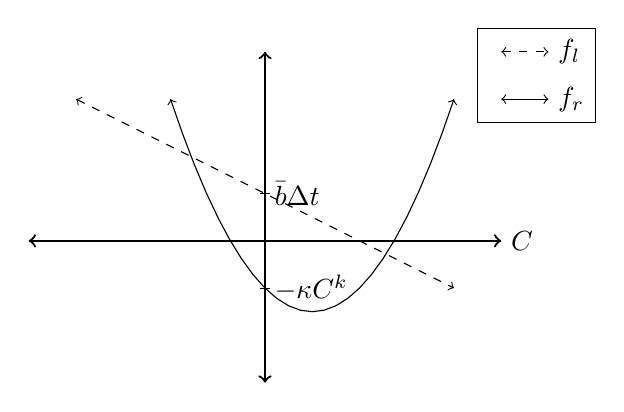
\begin{tikzpicture}[scale=0.6]
    \draw[<->, thick] (-5, 0) -- (5, 0);
    \draw[<->, thick] (0, -3) -- (0, 4); 
    \node[right] at (5, 0) {$C$};
    \node[above] at (0, 4) {};

    \draw[<->, domain=-2:4] plot (\x, {0.5*\x*\x - \x - 1});
    \draw (-0.1, -1) -- (0.1, -1);
    \node[right] at (0, -1) {$-\kappa C^{k}$};

    \draw[<->, dashed, domain=-4:4] plot (\x, {-0.5*\x+1});
    \draw (-0.1, 1) -- (0.1, 1); 
    \node[right] at (0, 1) {$\bar{b} \Delta t$};

    \draw (7, 2.5) -- (4.5, 2.5) -- (4.5, 4.5) -- (7, 4.5) -- (7, 2.5);
    \draw[<->, dashed] (5, 4) -- (6, 4);
    \node[right] at (6, 4) {$f_l$};
    \draw[<->] (5, 3) -- (6, 3);
    \node[right] at (6, 3) {$f_r$};

  \end{tikzpicture}
  &
  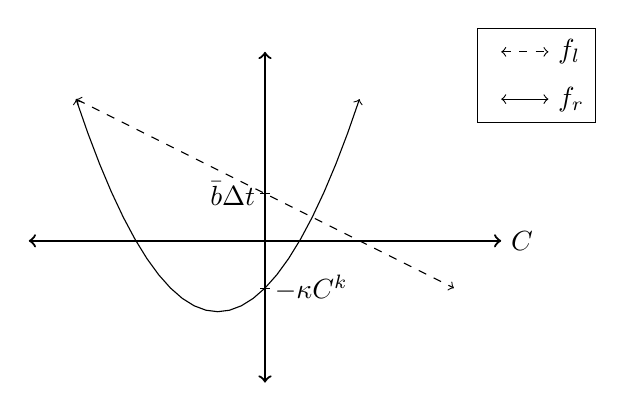
\begin{tikzpicture}[scale=0.6]
    \draw[<->, thick] (-5, 0) -- (5, 0);
    \draw[<->, thick] (0, -3) -- (0, 4); 
    \node[right] at (5, 0) {$C$};
    \node[above] at (0, 4) {};

    \draw[<->, domain=-4:2] plot (\x, {0.5*\x*\x + \x - 1});
    \draw (-0.1, -1) -- (0.1, -1);
    \node[right] at (0, -1) {$-\kappa C^{k}$};

    \draw[<->, dashed, domain=-4:4] plot (\x, {-0.5*\x+1});
    \draw (-0.1, 1) -- (0.1, 1); 
    \node[left] at (0, 1) {$\bar{b} \Delta t$};

    \draw (7, 2.5) -- (4.5, 2.5) -- (4.5, 4.5) -- (7, 4.5) -- (7, 2.5);
    \draw[<->, dashed] (5, 4) -- (6, 4);
    \node[right] at (6, 4) {$f_l$};
    \draw[<->] (5, 3) -- (6, 3);
    \node[right] at (6, 3) {$f_r$};
  \end{tikzpicture}
  \\
  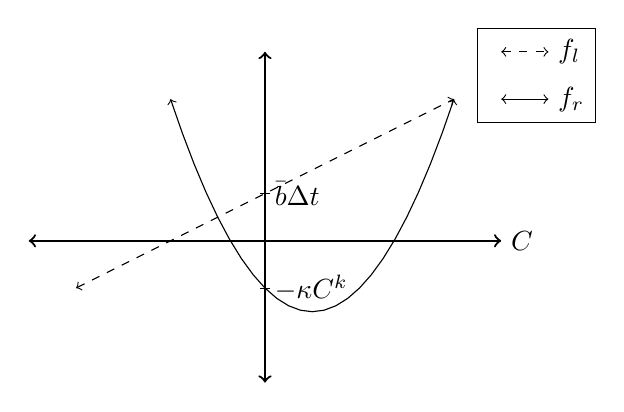
\begin{tikzpicture}[scale=0.6]
    \draw[<->, thick] (-5, 0) -- (5, 0);
    \draw[<->, thick] (0, -3) -- (0, 4); 
    \node[right] at (5, 0) {$C$};
    \node[above] at (0, 4) {};

    \draw[<->, domain=-2:4] plot (\x, {0.5*\x*\x - \x - 1});
    \draw (-0.1, -1) -- (0.1, -1);
    \node[right] at (0, -1) {$-\kappa C^{k}$};

    \draw[<->, dashed, domain=-4:4] plot (\x, {0.5*\x+1});
    \draw (-0.1, 1) -- (0.1, 1); 
    \node[right] at (0, 1) {$\bar{b} \Delta t$};

    \draw (7, 2.5) -- (4.5, 2.5) -- (4.5, 4.5) -- (7, 4.5) -- (7, 2.5);
    \draw[<->, dashed] (5, 4) -- (6, 4);
    \node[right] at (6, 4) {$f_l$};
    \draw[<->] (5, 3) -- (6, 3);
    \node[right] at (6, 3) {$f_r$};
  \end{tikzpicture}
  & 
  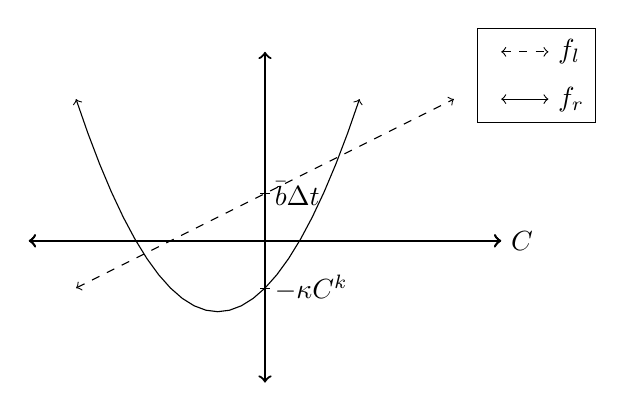
\begin{tikzpicture}[scale=0.6]
    \draw[<->, thick] (-5, 0) -- (5, 0);
    \draw[<->, thick] (-5, 0) -- (5, 0);
    \draw[<->, thick] (0, -3) -- (0, 4); 
    \node[right] at (5, 0) {$C$};
    \node[above] at (0, 4) {};

    \draw[<->, domain=-4:2] plot (\x, {0.5*\x*\x + \x - 1});
    \draw (-0.1, -1) -- (0.1, -1);
    \node[right] at (0, -1) {$-\kappa C^{k}$};

    \draw[<->, dashed, domain=-4:4] plot (\x, {0.5*\x+1});
    \draw (-0.1, 1) -- (0.1, 1); 
    \node[right] at (0, 1) {$\bar{b} \Delta t$};

    \draw (7, 2.5) -- (4.5, 2.5) -- (4.5, 4.5) -- (7, 4.5) -- (7, 2.5);
    \draw[<->, dashed] (5, 4) -- (6, 4);
    \node[right] at (6, 4) {$f_l$};
    \draw[<->] (5, 3) -- (6, 3);
    \node[right] at (6, 3) {$f_r$};
  \end{tikzpicture}
\end{tabular}
\caption{Graph of $f_l = \left( C \right)^2 + \left(\kappa - C^{k}\right)C - \kappa C^{k}$ and $f_r =  \left(\bar{b} - \bar{a} C \right) \Delta t$ for all four possible cases.
  Notice that because $-\kappa C^{k} < 0$ and $\bar{b} \Delta t > 0$ for all realistic parameter values the two functions will always intersect in the positive $C$ region.
  The top left graph is for $\bar{a} > 0$ and $\kappa - C^k < 0$.
  The top right graph is for $\bar{a} > 0$ and $\kappa - C^k > 0$.
  The bottom left graph is for $\bar{a} < 0$ and $\kappa - C^k < 0$.
  The bottom right graph is for $\bar{a} < 0$ and $\kappa - C^k > 0$.
}
\label{fig:proof_pos_sol}
\end{figure}
  
To determine which branch of (\ref{eq:Cquad}) to use, we look at the function logically.
If we know that one positive solution will always exist then the only branch for that to occur is the positive branch.
This is because the square root term, $\sqrt{b^2 -4c}$ will never be negative.
The addition of two negative numbers cannot result in a positive solution therefore the positive branch must be used for the positive solution that we desire.

Now that computable solutions for $M$ and $C$ at a single time step have been found, an algorithm to solve for the next time step can be established.
Algorithm \ref{alg:iterateCM} shows the organization of solving (\ref{equ:C_fixed_point} - \ref{equ:M_fixed_point}). 
\begin{algorithm}
  \KwData{$M^{k}$, $C^{k}$ are vectors with values from the previous time step and $p = 0$. }
  \Begin
  {
    Let $M^{(p=0)} = M^{k}$ and $C^{(p=0)} = C^{k}$\;
    \While{Convergence is not achieved } 
    {
        Solve $A^{(p)} M^{(p+1)} = \frac{1}{\Delta t}M^{(p)}$\;
        Solve $C^{(p+1)} = \frac{1}{2} \left( b \pm \sqrt{b^2 - 4c} \right)$\;
        Check convergence, (\ref{equ:iteration_convergence}\; 
        Let $p = p + 1 $\;
    }
    Let $P := p$\;
    Let $M^{(k+1)} = M^{(P)}$ and $C^{(k+1)} = C^{(P)}$\;
  }
  \caption{Algorithm for the fully-implicit solving of (\ref{equ:model_system}) }
  \label{alg:iterateCM}
\end{algorithm}

Note that Algorithm \ref{alg:iterateCM} actually describes both a fully-implicit and a semi-implicit method for solving (\ref{equ:model_system}). 
Recall that the final number of iterations is recorded as $P$, if $P = 1$ then only a single iteration of the algorithm is applied, which correlates to the behaviour of the semi-implicit method.
This can be produced by selecting a sufficiently large enough tolerance so that the convergence check, (\ref{equ:iteration_convergence}), is always resolved after the first iteration.
The resulting semi-implicit method is effectively the method described in \cite{sirca2012computational}, which was first introduced in \cite{eberl2007finite}.



